%%
%% Class homework & solution template for latex
%% Alex Ihler
%%
\documentclass[twoside,11pt]{article}
\usepackage{amsmath,amsfonts,amssymb,amsthm}
\usepackage{graphicx,color}
\usepackage{verbatim,url}
\usepackage{listings}
\usepackage{hyperref}
\usepackage{upquote}
\usepackage[T1]{fontenc}
%\usepackage{lmodern}
\usepackage[scaled]{beramono}
%\usepackage{textcomp}

% Directories for other source files and images
\newcommand{\bibtexdir}{../bib}
\newcommand{\figdir}{fig}

\newcommand{\E}{\mathrm{E}}
\newcommand{\Var}{\mathrm{Var}}
\newcommand{\N}{\mathcal{N}}
\newcommand{\matlab}{{\sc Matlab}\ }

\setlength{\textheight}{9in} \setlength{\textwidth}{6.5in}
\setlength{\oddsidemargin}{-.25in}  % Centers text.
\setlength{\evensidemargin}{-.25in} %
\setlength{\topmargin}{0in} %
\setlength{\headheight}{0in} %
\setlength{\headsep}{0in} %

\renewcommand{\labelenumi}{(\alph{enumi})}
\renewcommand{\labelenumii}{(\arabic{enumii})}

\theoremstyle{definition}
\newtheorem{MatEx}{M{\scriptsize{ATLAB}} Usage Example}

\definecolor{comments}{rgb}{0,.5,0}
\definecolor{backgnd}{rgb}{.95,.95,.95}
\definecolor{string}{rgb}{.2,.2,.2}
\lstset{language=Matlab}
\lstset{basicstyle=\small\ttfamily,
        mathescape=true,
        emptylines=1, showlines=true,
        backgroundcolor=\color{backgnd},
        commentstyle=\color{comments}\ttfamily, %\rmfamily,
        stringstyle=\color{string}\ttfamily,
        keywordstyle=\ttfamily, %\normalfont,
        showstringspaces=false}
\newcommand{\matp}{\mathbf{\gg}}




\begin{document}

Here is the system:
\begin{figure}[h]
\centering
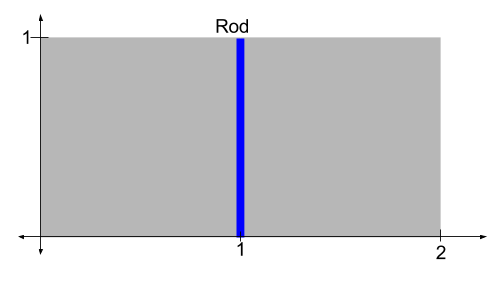
\includegraphics[height=1.5in]{PlateAndRod.png}
\caption{A plate with a rod in the middle}
\end{figure}

I am using the sequential splitting technique described in section 2.1 of \href{http://www.sciencedirect.com/science/article/pii/S0307904X07001606}{this paper}
\\
Let R represent the plate without the rod\\
Let V represent the plate with the rod temperature as a boundary condition\\
Let F be the final temperature of the plate with the plate and rod interacting\\
I am assuming F = R + V\\
\\
The diffusion equation used will be the following:
\[
\frac{\partial F}{\partial t} = \alpha_{plate} (\frac{\partial^2 F}{\partial x^2} + \frac{\partial^2 F}{\partial y^2})
\]
I will let the initial condition be 
\[
F(x,y,0)=20x(x-2)y(y-1)
\]
The boundary conditions will be as follows:
\[
F(0,y,t)=F(2,y,t)=F(x,0,t)=F(x,1,t)=0
\]

For the rod $u(y,t)$, I will assume its diffusion equation is as follows
\[
\frac{\partial u}{\partial t} = \alpha_{rod} \frac{\partial^2 u}{\partial y^2}
\]
The initial condition will be $u(y,0)=F(1,y,0)$\\
The boundary conditions will be $u(0,t)=u(1,t)=0$\\
\\
When computing R, I will use the same differential as F and the same boundary conditions. \\
When computing V, I will impose the condition that $V(1,y,t)=u(y,t)$\\
\\
The pseudo-code and implementation are in the attached mathematica notebook.



\end{document}
